%%
%% This is file `sample-manuscript.tex',
%% generated with the docstrip utility.
%%
%% The original source files were:
%%
%% samples.dtx  (with options: `all,proceedings,bibtex,manuscript')
%% 
%% IMPORTANT NOTICE:
%% 
%% For the copyright see the source file.
%% 
%% Any modified versions of this file must be renamed
%% with new filenames distinct from sample-manuscript.tex.
%% 
%% For distribution of the original source see the terms
%% for copying and modification in the file samples.dtx.
%% 
%% This generated file may be distributed as long as the
%% original source files, as listed above, are part of the
%% same distribution. (The sources need not necessarily be
%% in the same archive or directory.)
%%
%%
%% Commands for TeXCount
%TC:macro \cite [option:text,text]
%TC:macro \citep [option:text,text]
%TC:macro \citet [option:text,text]
%TC:envir table 0 1
%TC:envir table* 0 1
%TC:envir tabular [ignore] word
%TC:envir displaymath 0 word
%TC:envir math 0 word
%TC:envir comment 0 0
%%
%% The first command in your LaTeX source must be the \documentclass
%% command.
%%
%% For submission and review of your manuscript please change the
%% command to \documentclass[manuscript, screen, review]{acmart}.
%%
%% When submitting camera ready or TAPS, please change the command
%% to \documentclass[sigconf]{acmart} or whichever template is required
%% for your publication.
%%
%%
\documentclass[manuscript,screen,nonacm]{acmart}
%%
%% \BibTeX command to typeset BibTeX logo in the docs
\AtBeginDocument{%
  \providecommand\BibTeX{{%
    Bib\TeX}}}

% Force one-sided layout with uniform margins
\usepackage{geometry}
\geometry{
  left=1in,
  right=1in,
  top=1in,
  bottom=1in,
  asymmetric
}

\usepackage{array}
\usepackage{placeins}
\usepackage{algorithm}
\usepackage{algorithmic}
\usepackage{booktabs} % Required for toprule, midrule, bottomrule
% Prefer vector (PDF) charts when available; fallback to PNG/JPG.
\usepackage{ifthen}
\newcommand{\includebestgraphics}[2][]{%
    % #1 = optional includegraphics options, #2 = base filename without extension
    \IfFileExists{#2.pdf}{%
        \includegraphics[#1]{#2.pdf}%
    }{\IfFileExists{#2.png}{%
        \includegraphics[#1]{#2.png}%
    }{\IfFileExists{#2.jpg}{%
        \includegraphics[#1]{#2.jpg}%
    }{%
        \PackageWarning{includegraphics}{File `#2' not found with .pdf/.png/.jpg extensions}%
    }}}
}
%% Rights management information.  This information is sent to you
%% when you complete the rights form.  These commands have SAMPLE
%% values in them; it is your responsibility as an author to replace
%% the commands and values with those provided to you when you
%% complete the rights form.
\setcopyright{acmlicensed}
\copyrightyear{2018}
\acmYear{2018}
\acmDOI{XXXXXXX.XXXXXXX}
%% These commands are for a PROCEEDINGS abstract or paper.
% \acmConference[Conference acronym 'XX]{Make sure to enter the correct
%   conference title from your rights confirmation email}{June 03--05,
%   2018}{Woodstock, NY}
%%
%%  Uncomment \acmBooktitle if the title of the proceedings is different
%%  from ``Proceedings of ...''!
%%
%%\acmBooktitle{Woodstock '18: ACM Symposium on Neural Gaze Detection,
%%  June 03--05, 2018, Woodstock, NY}
% \acmISBN{978-1-4503-XXXX-X/2018/06}


%%
%% Submission ID.
%% Use this when submitting an article to a sponsored event. You'll
%% receive a unique submission ID from the organizers
%% of the event, and this ID should be used as the parameter to this command.
%%\acmSubmissionID{123-A56-BU3}

%%
%% For managing citations, it is recommended to use bibliography
%% files in BibTeX format.
%%
%% You can then either use BibTeX with the ACM-Reference-Format style,
%% or BibLaTeX with the acmnumeric or acmauthoryear sytles, that include
%% support for advanced citation of software artefact from the
%% biblatex-software package, also separately available on CTAN.
%%
%% Look at the sample-*-biblatex.tex files for templates showcasing
%% the biblatex styles.
%%

%%
%% The majority of ACM publications use numbered citations and
%% references.  The command \citestyle{authoryear} switches to the
%% "author year" style.
%%
%% If you are preparing content for an event
%% sponsored by ACM SIGGRAPH, you must use the "author year" style of
%% citations and references.
%% Uncommenting
%% the next command will enable that style.
%%\citestyle{acmauthoryear}


%%
%% end of the preamble, start of the body of the document source.
\begin{document}

%%
%% The "title" command has an optional parameter,
%% allowing the author to define a "short title" to be used in page headers.
\title[]{Guiding End-Users Toward Software Reuse: An Evaluation of Automated Assistance in Block-Based Programming for Chemistry Laboratory Automation}

%%
%% The "author" command and its associated commands are used to define
%% the authors and their affiliations.
%% Of note is the shared affiliation of the first two authors, and the
%% "authornote" and "authornotemark" commands
%% used to denote shared contribution to the research.
\author{Anne-Marie Rommerdahl}
\affiliation{%
 \institution{SDU}
 \city{Odense}
 \country{Denmark}}
\email{anrom25@student.sdu.dk}

\author{Jeremy Alexander Ramírez Galeotti}
\affiliation{%
 \institution{SDU}
 \city{Odense}
 \country{Denmark}}
\email{jeram25@student.sdu.dk}

\author{Dimitrios Dafnis}
\affiliation{%
 \institution{SDU}
 \city{Odense}
 \country{Denmark}}
\email{didaf25@student.sdu.dk}

\author{Nasifa Akter}
\affiliation{%
 \institution{SDU}
 \city{Copenhagen}
 \country{Denmark}}
\email{naakt23@student.sdu.dk}

\author{Mohammad Hosein Kardouni}
\affiliation{%
 \institution{SDU}
 \city{Odense}
 \country{Denmark}}
\email{mokar25@student.sdu.dk}



%%
%% By default, the full list of authors will be used in the page
%% headers. Often, this list is too long, and will overlap
%% other information printed in the page headers. This command allows
%% the author to define a more concise list
%% of authors' names for this purpose.
\renewcommand{\shortauthors}{}

%%
%% The abstract is a short summary of the work to be presented in the
%% article.
\begin{abstract}


\noindent\textbf{\textit{Abstract}—Background: End-users who program collaborative robots for laboratory automation often create repetitive code because they struggle to recognize opportunities for reuse. While block-based programming environments provide accessible interfaces, they do not actively guide users toward creating reusable components.}

\noindent\textbf{Objective: This study investigates whether automated guidance can help end-users recognize and apply code reuse practices. We developed the Reuse Assistant, a feature that automatically detects duplicate code sequences in OpenRoberta and guides users to create reusable custom blocks through visual highlighting and one-click refactoring.}

\noindent\textbf{Methods: Through a within subjects study with 10 participants from the chemistry domain, we evaluated the feature's impact on performance, usability, and perceived workload.}

\noindent\textbf{Results: Automated guidance increased reuse adoption from 0\% in the standard environment to 100\% with the Reuse Assistant. The feature achieved high usability scores (SUS mean: 84.1) and imposed minimal cognitive burden (NASA-TLX mean: 1.88). A significant order effect revealed that prior manual experience helps users appreciate automation benefits.}

\noindent\textbf{Conclusions: Our findings extend the Attention Investment Model and Learning Barriers Framework, demonstrating that proactive assistance can transform feature adoption from a high-cost investment to a low-cost opportunistic choice. The results provide design principles for developing end-user programming tools that effectively guide domain experts without adding complexity.}
\end{abstract}
%%
%% This command processes the author and affiliation and title
%% information and builds the first part of the formatted document.
\settopmatter{printacmref=false, printccs=false, printfolios=true} % Remove ACM Reference Format and copyright info
\renewcommand\footnotetextcopyrightpermission[1]{} % Remove copyright footer
\maketitle
%%
%% The code below should be generated by the tool at
%% https://dl.acm.org/ccs.cfm
%% Please copy and paste the code instead of the example below.
%%
% \begin{CCSXML}
% <ccs2012>
% <concept>
% <concept_id>10011007.10011006.10011008</concept_id>
% <concept_desc>Software and its engineering~General programming languages</concept_desc>
% <concept_significance>500</concept_significance>
% </concept>
% <concept>
% <concept_id>10003456.10003457.10003521.10003525</concept_id>
% <concept_desc>Social and professional topics~History of programming languages</concept_desc>
% <concept_significance>300</concept_significance>
% </concept>
% </ccs2012>
% \end{CCSXML}

% \ccsdesc[500]{Software and its engineering~General programming languages}
% \ccsdesc[300]{Social and professional topics~History of programming languages}

%%
%% Keywords. The author(s) should pick words that accurately describe
%% the work being presented. Separate the keywords with commas.
\keywords{end-user development, block-based programming, code reuse, automated guidance, laboratory automation, collaborative robots, usability, attention investment model, learning barriers}


\section{Introduction}

Software reuse is a fundamental practice in software engineering, enabling developers to build on existing solutions rather than 
writing code from scratch. However, end-users who program collaborative robots (cobots) for laboratory automation often lack the 
knowledge to recognize and apply reuse opportunities. This problem is particularly acute in domains like chemistry, where scientists 
need to automate repetitive experimental procedures but have limited programming expertise.

Block-based programming environments such as OpenRoberta Lab provide accessible interfaces for programming robots, but they do not 
actively guide users toward creating reusable components. As a result, end-users frequently produce long, repetitive programs that are 
difficult to maintain and modify. When experimental protocols change, users must manually update code in multiple locations, increasing 
the risk of errors and discouraging adoption of automation features.

This study addresses the question: Can automated guidance help end-users recognize and apply code reuse in block-based programming? 
We developed the Reuse Assistant, a feature that automatically detects duplicate code sequences and guides users to create reusable custom 
blocks through visual highlighting and one-click refactoring. Through a within subjects study with 10 participants from the chemistry domain, 
we evaluated whether proactive automated assistance can overcome the barriers that prevent end-users from adopting reuse practices.

Our investigation examined three research questions: (1) Can the Reuse Assistant improve end-user performance? (2) Is the Reuse Assistant 
sufficiently usable for end-users? (3) What is the perceived workload when using the Reuse Assistant? The results showed that automated 
guidance increased reuse adoption from 0\% to 100\%, achieved high usability scores (SUS mean: 84.1), and imposed minimal cognitive 
burden (NASA-TLX mean: 1.88).

The contributions of this work are both theoretical and practical. We extend the Attention Investment Model by demonstrating that 
proactive assistance can transform feature adoption from a high-cost investment to a low-cost opportunistic choice. 
We also extend Ko et al.'s Learning Barriers Framework by showing that the selection barrier dominates in block-based environments 
for end-users. From a practical perspective, our results demonstrate that simple design principles (visual highlighting, one-click acceptance,
immediate feedback) can effectively guide end-users without adding complexity, as evidenced by high usability and low workload scores.

\section{Background and Related Work}
\label{sec:background_relatedWork}
%% ---- Background ----
%% 1 Background abt. reuse. What is it, and why is it important? (anne)
%% 2 What is the current state of 'reuse' for low-code? Anne paragraph (anne)
%% 3 In what ways have different low-code tools tackled 'reuse'? We look at different low-code tools, not just block-based ones. What are the strengths and weaknesses of their approach to reuse? MAKE SURE TO MENTION TOOLS BY NAME! (dimitris)
%% 4 Now we look at block-based tools for robots (for example, scratch, VEXcode GO, OpenRoberta). How do they tackle reuse? (jeremy + Mohamad)
%% 5 Based on the identified weaknesses in current practices for reuse, we propose our own idea (explain how it's gonna work) (Nasifa)

%% ----Re-done intro----
Software reuse is a broad term, that refers to the practice of reusing previously written code, rather than coding from scratch. It is such an important part of software engineering, that one of the ways to measure the quality of software is by its 'Reusability'\cite{SoftwareArchitectureInPractice}, i.e. the degree to which the application or its components can be reused. 
There are multiple benefits to practicing reuse in software engineering. One developer could save time by using another developer's reusable component, rather than coding their own. The developer avoids both the work of writing the syntax and designing the logic of the component. The developer can design their own reusable components, keeping all the logic in one place, which can then be tested thoroughly. However, despite reuse being an important practice in software engineering, there is still a limited focus on this practice when it comes to low-code development platforms (LCDP).

%%--from here: what reuse is there for low-code? What research? IN GENERAL
%%-- Then, what tools? examples of how tools tackle reuse
%%-- Then, what tools for blocks and robots? How do they tackle reuse? What are their strengths/weaknesses/limitations? MAKE SURE TO MENTION BY NAME!!
%%-- Show the tool we'll be working on (what does it do for reuse, and weaknesses).
%%-- Based on all that, what is our idea? What gap is it, we're addressing and how?
%% ---------------------
A study from 2021 studied several low-code platforms (LCPs), in order to identify characteristic features of LCPs. The identified features were presented according to how frequent they occured, with domain-specific reference artifacts being categorized as 'rare'. Most studied systems offered catalogs of "reusable functions or examples of predefined processes", but they were found to be generic, or have a limited scope\cite{LowCodePlatform}. This lack of focus on promoting reuse may impact the so-called 'Citizen Developers', who have little or no coding knowledge, and whom may then miss out on the benefits of reuse. Lin and Weintrop (2021) noted that most existing research on block-based programming focuses on supporting the transition to text-based languages rather than exploring how features within BBP environments \cite{Lin2021Landscape}, such as abstraction or reuse, can enhance learning outcomes.

There have been proposed some ideas on how to promote reuse for LCPs, such as the templating language OSTRICH, developed for model-driven low-code platform OutSystems\cite{OSTRICH}. OSTRICH is designed to assist the end-user in making use of OutSystems' available templates, by abstracting and parameterizing the templates. However, OSTRICH only supports the top nine most used production-ready screen templates, and does not allow the end-user to create and save their own templates, or re-apply a template which they have customized. Another approach focused on enabling the reuse of models, by providing recommendations to the end-user, based on the models stored in a graph acting as a repository. While the graph allows end-users to reuse their own models, there is no mention of guiding the user towards reusing their own models.

%Low code platform tools that focus on reuse
%[x does this, y does that, but a common trend seen in all of them is the almost nonexistent guidance towards using these features. If a user doesnt know/care about reuse, that mentality is never challenged.]
Several popular low-code development platforms (LCDPs) provide different kinds of support for reuse. Webflow\cite{webflow}, a LCDP for responsive websites, offers the ability to create reusable components and UI kits, which can be reused across multiple pages and projects. 
Mendix\cite{mendix} and OutSystems offer even more functionality to support reuse, offering several ways to end-users to share their code with each other, and offering pre-made components. Both of these platforms also utilize AI to enhance reuse. Outsystems provides AI suggestions to spot and create reusable pieces, while Mendix uses AI to suggest the best solutions and components for specific tasks. However, for both of these platforms, the AI suggestions provided are not always accurate to successfully guide the end-user to create custom reusable components.\\
%Mendix\cite{mendix} also offers the ability for end-users to create reusable building blocks, and these can be shared with others. The platform provides AI suggestions to spot and create reusable pieces, empowering even beginners to build complex apps while keeping reuse simple and widespread. This tool does offer guidance for the end-users to create custom reusable components through its AI suggestions, a lot of times these suggestions are not accurate enough*****(HOW do we know whether it's accurate???)    ***(How do we know this? What makes it 'accurate'?**)****
% Webflow - Despite all of the useful features that this tools has, it does not provide guidance to the end-users to create custom reusable components. % which is the key feature of our project.
% Mendix - This tool does offer guidance for the end-users to create custom reusable components through its AI suggestions, a lot of times these suggestions are not accurate enough (how do we know this??**).
In order to analyze how block-based robotics environments address reuse, 4 representative platforms were compared: mBlock, MakeCode, SPIKE LEGO, VEXcode GO and Open Roberta. The comparison focused on three main dimensions of reuse: structural reuse (through user-defined blocks or functions), social reuse (through sharing or remixing existing projects), and interoperable reuse (through import/export capabilities).
\begin{table}[H]
  \small   
  \caption{Block Based Robotics Environments Reuse Support}
  \label{tab:reuse_support}
  \begin{tabular}{lcccc}
    \toprule
    Platform & Structural Reuse & Social Reuse & Interoperable Reuse & Reuse Support \\
    \midrule
    VEXcode GO    & X & X &  & Medium \\
    mBlock        & X & X & X & Medium \\
    MakeCode      & X & X & X & Medium \\
    Spike Lego    & X &  & X & Low \\
    Open Roberta  &  & X &  & Low \\
    \bottomrule
  \end{tabular}
\end{table}
In this context, “reuse support” represents a scale that measures how effectively each platform facilitates reuse-related features. High reuse support indicates that users can easily create, share, and adapt existing components or projects. Medium reuse support suggests that some reuse mechanisms are available but limited in scope or flexibility. Low reuse support implies that the platform provides only minimal or restricted features to promote reuse.

As shown in Table 1, although these platforms include reusability features, they are quite limited, as none of them provide users with clear guidance on how to use these tools effectively, which restricts their ability to fully leverage them.\\\\
A study by Techapalokul and Tilevich (2019) suggests that supporting mechanisms for reusing smaller, modular pieces of code can enhance programmer productivity, creativity and learning outcomes. 
%Techapalokul and Tilevich (2019) proposed extending the Scratch programming environment with facilities for reusing individual custom blocks to promote procedural abstraction and improve code quality. They observed that while Scratch enables remixing of entire projects, it lacks mechanisms for reusing smaller, modular pieces of code. Their work suggests that supporting such fine-grained code reuse could enhance programmer productivity, creativity, and learning outcomes. Building on this idea, our project applies similar principles within the OpenRoberta environment by automating the detection of duplicate code segments and guiding users toward creating reusable custom blocks.
Adler et al. (2021) introduced a search-based refactoring approach to improve the readability of Scratch programs by automatically applying small code transformations, such as simplifying control structures and splitting long scripts. Their findings demonstrated that automated refactoring can significantly enhance code quality and readability for novice programmers. Building upon this concept, our project applies similar principles in the OpenRoberta environment, focusing on detecting duplicate code segments and guiding users toward creating reusable custom blocks to promote modularity and abstraction.\cite{Adler2021Improving}.

Existing block-based environments provide mechanisms for reuse, but lack intelligent support to help users recognize and apply reuse in practice. To address this gap, our project introduces a guided reuse assistant within the Open Roberta Lab environment.
The tool is designed to help users identify and apply reuse more easily while creating their robot programs. It works by automatically scanning a user’s block-based program to detect repeated code segments in the workspace. The system visually highlights the found duplicates, drawing the user’s attention to patterns that could be simplified.

The tool also offers the functionality to create the custom block for the end-user, by identifying the small differences between the repeated parts (such as numbers, variables, or parameters) and turning these differences into inputs for the new block. The tool automatically replaces all relevant duplicate sequences with the new custom block.

%When repeated blocks are detected, the assistant suggests creating a reusable custom block (function). It then helps the user generate this new block by identifying the small differences between the repeated parts (such as numbers, variables, or parameters) and turning these differences into inputs for the new block. After the user confirms, the system automatically replaces all the repeated sequences with calls to the newly created reusable block.

By combining ideas from procedural abstraction (organizing code into meaningful, reusable parts) and automated refactoring (improving code through intelligent transformations), our tool aims to make block-based programming more structured and efficient.
It encourages users to build programs that are modular and easier to maintain, helps reduce unnecessary repetition, and supports learning by making the concept of reuse clear and hands-on.
%In summary, our work bridges the gap between existing theoretical approaches to software reuse and their real-world application in block-based programming environments. Through this guided and semi-automated approach, we aim to make reuse visible, understandable, and practical for end-users working in Open Roberta.
\section{Study Design}
\label{sec:study_design}

Following the Design Science methodology, our study is structured into three main phases: problem investigation to define goals, treatment design to specify the artifact requirements, and treatment validation to assess the artifact's performance in a controlled environment.

\subsection{Problem Investigation}
\label{subsec:prob_investigation}

\subsubsection{Problem Context and Motivation}

End-user development (EUD) for collaborative robots (cobots) presents unique challenges, particularly for users without formal programming training. In domains such as chemistry laboratories, educational robotics, and industrial settings, end-users need to program 
robots to perform specific tasks but often lack the software engineering knowledge to write maintainable, well-structured code.
In the domain of Chemistry, one of the most relevant and important tasks is performing experiments in labs in order to test a hypothesis, or to aid in the understanding of how chemicals react. 
Robots can be used in chemistry labs to automate experiments with great effect, as many experiments involve steps that are repetitive, and susceptible to human error, such as a step being overlooked, instructions being misread, etc. Automation of menial tasks will leave the chemists with more time for other work, and also comes with the added bonus of chemists not having to handle dangerous chemicals. 
One critical challenge in EUD is code reuse. Users frequently create repetitive code because they struggle to recognize duplicate patterns, lack knowledge about abstraction mechanisms, or find existing tools too complex to use effectively. This problem manifests in several ways: programs become unnecessarily long and difficult to maintain and small changes require modifications in multiple locations, increasing the risk of errors. 
Several  visual programming environments, like OpenRoberta Lab, don't provide assistance in identifying when code should be reused or how to extract repeated sequences into reusable components. As lab work in chemistry involves many repetitive tasks, these challenges can easily become an obstacle for the chemists, which may turn them away from using cobots, as the inconvenience outweighs the benefits.

\subsubsection{Stakeholder Analysis}

Chemists and lab technicians who use cobots for repetitive tasks such as sample preparation, dispensing, mixing, and quality control procedures. 
They possess deep domain expertise in chemistry but limited programming knowledge, often creating long, repetitive programs that become difficult to maintain when adapting experimental protocols. 
Their primary need is to quickly create and modify robot programs without becoming programming experts.


\subsection{Treatment Design}
\label{subsec:treatment_design}

To address the problem of code reuse in EUD for cobots, we have derived a set of requirements designed to contribute to the chemist's goal of creating maintainable and reusable robot programs.
Functionally, the artifact must be capable of automatically detecting duplicate or similar block sequences and visually highlighting these duplications within the user's workspace.
These requirements are necessarry to help the end-user recognize opportunities for reuse, that would otherwise go unnoticed. Once detected, the system must suggest the creation of reusable custom blocks, allowing the user to accept or reject these suggestions.
These signals are important, as they give the end-user control over the reuse process, allowing them to decide when and how to apply reuse in their programs.
Regarding non-functional requirements, the artifact must seamlessly integrate with the existing Open Roberta Lab environment to ensure a smooth user experience.
The interface should be intuitive for end-users, minimizing the learning curve and making it easy to understand and use the reuse features. Additionally, the artifact should not interfere with the existing workflow, allowing users to continue their programming tasks without disruption. Finally, clear visual feedback during the detection process is essential to help users understand what the system is doing and how to respond to its suggestions.


\subsubsection{Artifact Specification: The Reuse Assistant}
To satisfy the requirements above, we designed the Reuse Assistant as an extension of Open Roberta Lab. 

\subsubsection{Architecture}

The system enables the execution of block-based programs on a simulated cobot through a three-tier architecture, as illustrated in figure \ref{fig:architecture-zoom}. The workflow consists of the following stages:

\begin{enumerate}
    \item \textbf{Client Side (Open Roberta):} The user interacts with the Open Roberta UI to assemble block sequences. The Reuse Assistant operates at this layer, analyzing blocks in real-time. Upon execution, the client generates specific data structures ("Generated Headers") representing the program logic.
    \item \textbf{Backend (Flask Server):} The client transmits these headers via HTTP POST requests to a Flask-based API Endpoint. A "Translator" component processes the data, mapping the abstract block definitions to concrete Python methods compatible with the robot's control logic.
    \item \textbf{Simulation (Mujoco):} The mapped methods trigger the execution of commands within the Mujoco Simulator, which renders the physical behavior of the cobot in the virtual environment.
\end{enumerate}



% Zoomed version of the architecture figure on its own page
\begin{figure}[p]
    \centering
    \phantomsection
    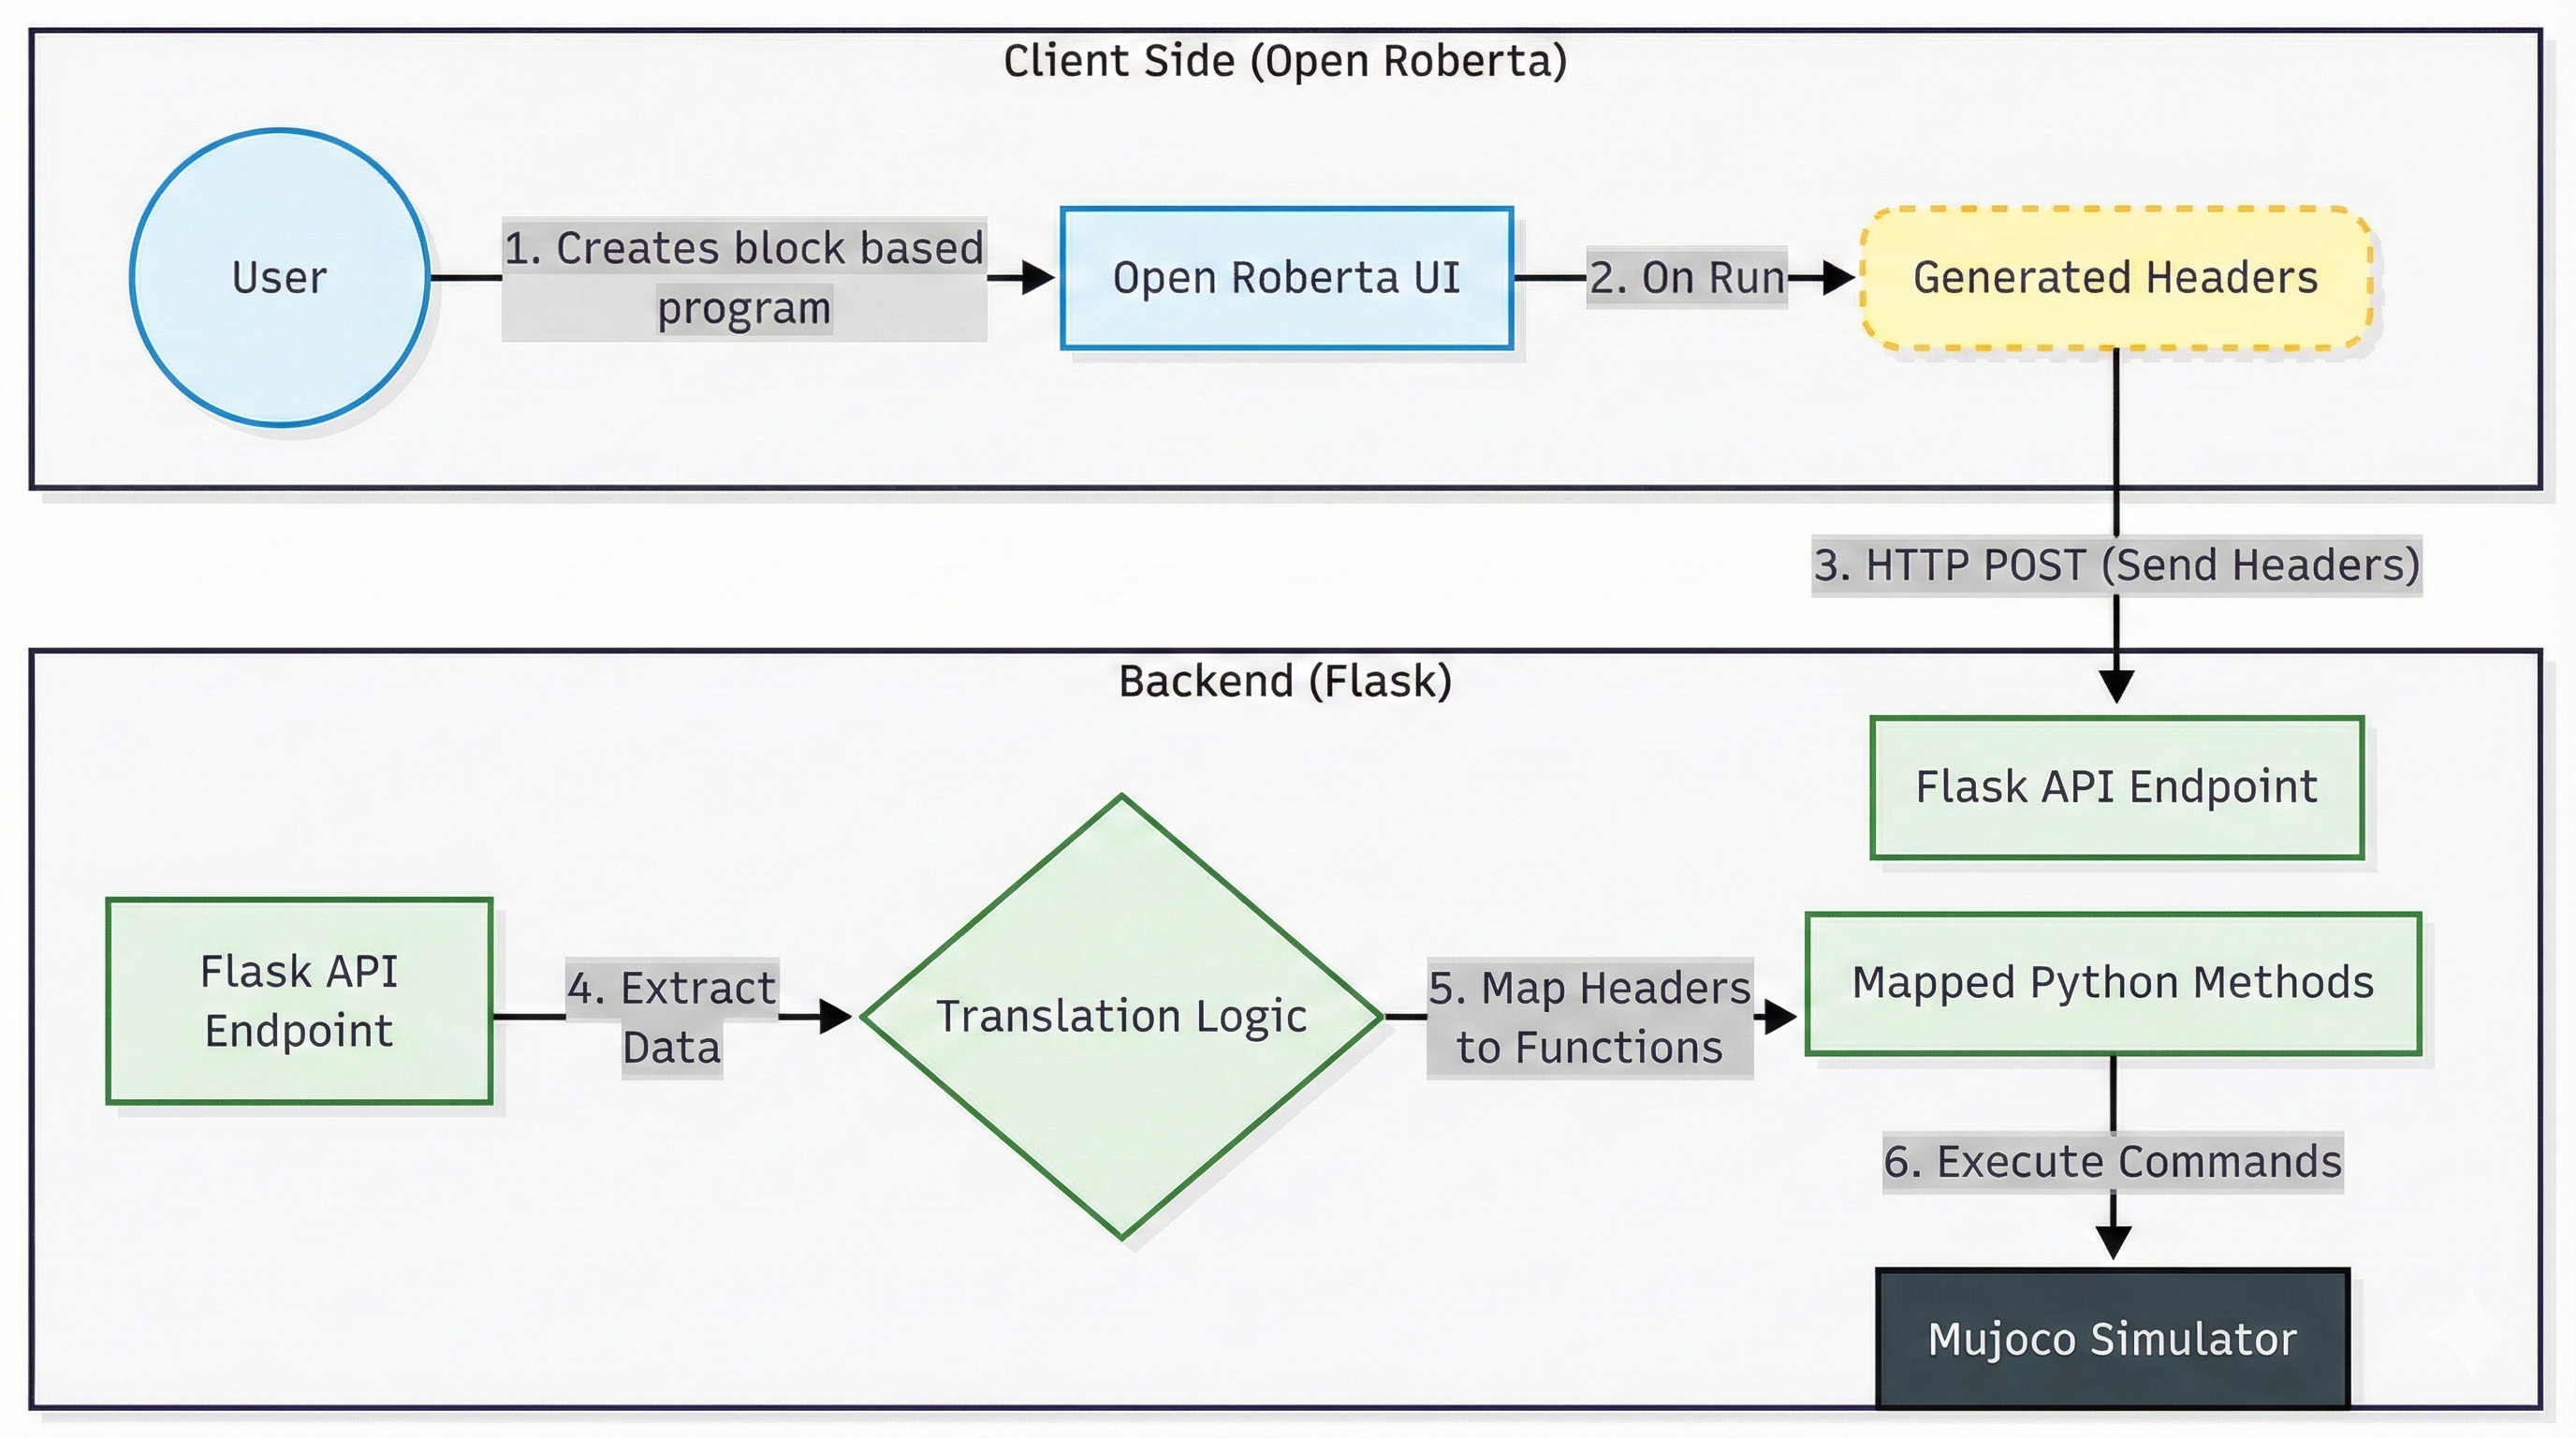
\includegraphics[height=0.9\textheight,keepaspectratio]{ArchitectureH2.png}
    \caption{System architecture}
    \label{fig:architecture-zoom}
    \Description{System architecture diagram showing the Client Side, Backend, and Simulator tiers in more detail.}
\end{figure}



\subsubsection{Detection Algorithm}
The approach is intentionally simple so it is easy to read
and to implement in a real block editor. The algorithm follows three main steps:
%\begin{itemize}
 %   \item \textbf{Linearization:} Convert the workspace into a flat, ordered list of blocks (preserving execution order).
 %   \item \textbf{Identify sequences:} Slide a window over the list and extract contiguous sequences whose length is at least a minimum (e.g. 3).
 %   \item \textbf{Pattern Matching:} Use the block type sequence as a key; group occurrences with the same key and report keys seen more than once.
%\end{itemize}

\begin{itemize}


    \item \textbf{Linearization:} First, the algorithm linearizes the block workspace into a sequential list of blocks. 
    
    \item \textbf{Identify sequences:} It then iterates through this list to identify all possible sequences of blocks that meet a minimum unique block type length requirement (three blocks) that can be repeated more than once.
    
    \item \textbf{Sequences Matching:} If the same sequence of block types is found more than once, it will be added to the CustomReusableCandidates list which will eventually be sorted by longest and most recent duplicated sequences. In the end the highest priority candidate gets returned.


\end{itemize}


The pseudocode below is short, explicit, and uses straightforward data structures (lists).

\begin{algorithm}[H]
\caption{Duplicate Sequence Detection}
\label{alg:detection_refined}
\begin{algorithmic}[1]
\REQUIRE Workspace, StartBlock \quad // user's block workspace
\REQUIRE MinimumSequenceLength = 3, MinimumDifferentBlockTypesInSequence = 3, MaxSequenceLength = 10 \quad
\ENSURE ReusableComponentCandidates \quad // list of repeated block sequences to return
\STATE Chain $=$ \textbf{buildLinearChain}(StartBlock) 
\STATE Sequences $=$ List$\langle$sequence$\rangle$ 

\FOR{startIndex = 0 \TO length(Chain) - 1} 
    \FOR{$sequenceLength = 1$ \TO $MaxSequenceLength$ }
        \STATE sequence $=$ Chain[startIndex \,..\, startIndex + sequenceLength - 1] 
        \STATE numberOfBlockTypesInSequence = getNumberOfDistinctBlockTypes(sequence)
        \IF{sequenceLength >= MinimumSequenceLength \textbf{ and } numberOfBlockTypesInSequence >= MinimumDifferentBlockTypesInSequence}
            \STATE Sequences.append(sequence) // record sequence occurrence
        \ENDIF
    \ENDFOR
\ENDFOR

\STATE ReusableComponentCandidates $= \{\text{Sequences} \mid occurrence \ge 2 \}$ 
\STATE sort ReusableComponentCandidates by (longest sequence length and most recent occurrence) 
\RETURN ReusableComponentCandidates[0] // Return highest priority candidate
\end{algorithmic}
\end{algorithm}


Algorithm 1. Illustrates the core logic for identifying duplicate block sequences

%\begin{algorithm}[H]
%\caption{Highlight duplicate sequences}
%\label{alg:detection_refined}
%\begin{algorithmic}[1]
%\REQUIRE Workspace, StartBlock \quad // user's block workspace
%\STATE SequenceToHighlight = DuplicateDetectionAlgorithm()
%\FOR{each SequenceToHighlight in Workspace}
%    \FOR{block in SequenceToHighlight} 
%        \STATE block.changeColor(GREEN) \quad // highlight duplicate blocks
%        \STATE alertUser("Duplicate sequence detected. Create reusable block?")
%        \IF{userConfirms()} 
%            \STATE createReusableBlockFromSequence(block)
%        \ENDIF
%    \ENDFOR
%   \ENDFOR
%\end{algorithmic}
%\end{algorithm}
%Algorithm 2. Illustrates when the system highlights duplicate sequences and alerts the user to create reusable blocks


%\begin{algorithm}[H]
%\caption{Event Listener}
%\label{alg:detection_refined}
%\begin{algorithmic}[1]
%\REQUIRE Workspace, StartBlock \quad // user's block workspace
%\STATE Window.eventListener("onEachEvent", HighlightDuplicateSequences,ResetBlockColors)
%\end{algorithmic}
%\end{algorithm}

%Algorithm 3. Illustrates how the detection algorithm is triggered on each user event in the workspace

% [TODO: Insert here your technical description from your original section 3.2.1. 
% Explain briefly the architecture, the detection algorithm, and how the UI works.]
\subsubsection{User Interface and Interaction}
The user interface is designed to be intuitive and non-disruptive. When the detection 
algorithm identifies a candidate, the system visually highlights the blocks on the canvas as illustrated in Figure \ref{fig:ui_interaction_highlight}. 
A non-blocking toast notification appears, prompting the user to confirm the refactoring. 
If confirmed, the system automatically generates the custom block definition in a dedicated 
workspace area (handling visibility via \texttt{revealDefinitionWorkspacePane}) and updates
the main workspace, replacing the redundant code with concise function calls as shown in Figure \ref{fig:ui_interaction_refactor}. 
This process abstracts the complexity of manual function creation, guiding the user toward modular 
design practices. 
After the user presses the run simulation button, the robot simulator of mujoco opens up and executes the commands provided by the user inside the Open Roberta workspace. This is illustrated in Figure \ref{fig:mujoco_simulator}.


% --- START: Split UI figures ---
\begin{figure}[htbp]
    \centering
    % Prefer vector PDF when available, fallback to PNG/JPG
    \includebestgraphics[width=0.85\linewidth]{highlight}
    \Description{A screenshot of the Open Roberta environment. Two identical sequences of blocks are highlighted. A pop-up message in the bottom right asks the user if they want to create a reusable block.}
    \caption{Reuse Assistant workflow: detection - the interface detects and highlights duplicate blocks by changing their color to green.}
    \label{fig:ui_interaction_highlight}
\end{figure}

\begin{figure}[htbp]
    \centering
    % Prefer vector PDF when available, fallback to PNG/JPG
    \includebestgraphics[width=0.85\linewidth]{custom_component}
    \Description{Screenshot showing the code after refactoring. The main program is now much shorter. A side panel shows the definition of the new custom block with parameters for coordinates.}
    \caption{Reuse Assistant workflow: refactoring - the automated refactoring result, showing the new custom block definition and the simplified main program.}
    \label{fig:ui_interaction_refactor}
\end{figure}

\begin{figure}[htbp]
    \centering
    % Prefer vector PDF when available, fallback to PNG/JPG
    \includebestgraphics[width=0.85\linewidth]{mujoco}
    \Description{Screenshot showing the code after refactoring. The main program is now much shorter. A side panel shows the definition of the new custom block with parameters for coordinates.}
    \caption{Mujoco robot simulator executing the commands from Open Roberta.}
    \label{fig:mujoco_simulator}
\end{figure}
% --- END: Split UI figures ---
\FloatBarrier
% -------------------------------------------------------------------------------------------------------------------------------------------------------------------
% validity threat here or in discussion?
% Treatment validation needs to be split into subsections "data gathering and analysis" How we gather the data and how we analyze them
%"Task execution" We need to explain what exactly will be the task
\subsection{Treatment Validation}
\label{subsec:treatment_validation}
The treatment validation for this study adopts a mixed-methods evaluation approach to assess 
the effectiveness of the proposed features for guiding users in creating custom reusable components (blocks) within 
the OpenRoberta environment. 

\subsubsection{Participant Recruitment}
A total of 10 participants were selected with similar level of expertise in block-based programming. 
Time constraints and resource availability have influenced the decision to limit the number of participants.
Participants were recruited from a diverse pool of individuals affiliated with the University of Southern Denmark and the broader chemistry community. 
This group of participants includes chemistry teachers, professional chemical engineers, and students currently enrolled in chemistry-intensive curricula. 
To ensure relevant practical expertise, the selection specifically targets those who frequently engage in laboratory environments. 
The experimental sessions were conducted across a range of environments to accommodate participant availability. 
Physical sessions took place within the chemistry laboratories at the University of Southern Denmark (SDU) as well as a private residential setting. 
For remote participants, sessions were administered virtually using Discord for communication and AnyDesk for remote desktop control.

\paragraph{Ethical Considerations and Sampling}
Prior to the commencement of the study, all participants are required to sign a consent form acknowledging their voluntary participation and granting permission for screen recording and data usage. 
It should be noted that this recruitment strategy constitutes \textit{convenience sampling}. As such, they may not represent the general population.
% -------------------------------------------------------------------------------------------------------------------------------------------------------------------
\subsubsection{Task Execution}
The participants were initially given a short introduction to the OpenRoberta UI, as well as the mujoco robot simulator. 
They then performed one task which is described by a set of pre-defined steps to perform. This task has been specifically designed to promote the reusability aspect.
The task is focused on the domain of chemistry, as it is modelled after a real lab experiment perfomed by chemistry students at SDU. 

The participants were instructed to program the robot to execute the following sequence of operations:

\begin{enumerate}
    \item Move the robot arm above mix cylinder
    \item Mix the chemistry ingredients
    \item Move the robot arm above the analysis pad
    \item Analyze the sample
    \item If the solution is analyzed (use if statement) then show a response message in the laptop’s screen 
    \item Place the following three objects into their corresponding slots in the chemistry equipment toolbox:
    \begin{itemize}
        \item Methanol cylinder
        \item Chloroform syringe
        \item Toluene syringe
    \end{itemize}
    \item Important notes for the participants:
    \begin{itemize}
        \item \textit{After placing an object to its slot in the toolbox \textbf{wait 2 seconds} before you move to pick a new one.}
        \item \textit{After placing the \textbf{chloroform syringe} to its slot, \textbf{move the robot arm up by 10 cm} before you move to pick the next chemistry object }
        \item \textit{Click the \textbf{play} button on the bottom right corner to start the simulation}
        \item \textit{Click the \textbf{reset} button on the bottom right corner to reset the scene of the robot simulator}
    \end{itemize}
\end{enumerate}

Most optimal solution pre-defined by the researchers:
 \begin{figure}[h]
     \centering
     \includegraphics[width=0.8\textwidth]{most optimal solution.png}
     \caption{The optimal solution implemented in OpenRoberta, utilizing a custom block for the object placement sequence.}
     \Description{Block-based program showing the optimal solution with a custom reusable block for placing chemistry objects into toolbox slots.}
     \label{fig:optimal_solution}
 \end{figure}

Instead of creating a long linear sequence of blocks, the most optimal solution utilizes a Custom Reusable Component to handle the repetitive action of placing an object to its corresponding slot inside the equipment toolbox. 
This approach not only reduces redundancy but also enhances code maintainability and readability, aligning with best practices in software development.

All the participants will try to complete the task using both the standard and the enhanced version of OpenRoberta. 
Half of the participants will begin using the enhanced version of OpenRoberta, while the other half will start with the standard version.
Participants’ interactions with the platform will be observed throughout the task.
Guidance will be provided from the researchers to the participants throughout the task.

% -------------------------------------------------------------------------------------------------------------------------------------------------------------------
\subsubsection{Data Gathering and Analysis}
Data collection focuses on both quantitative performance and qualitative feedback from participants:
\begin{enumerate}
    \item \textbf{Task Completion Time:} Measured for both versions (Enhanced and Original) to compare performance across groups. Statistical analysis included paired t-tests to evaluate within-group improvements and between-group comparisons to identify order effects (carryover effects).
    \item \textbf{Solution Accuracy:} Evaluated by comparing participant solutions against the optimal reference solution. The primary metric was the voluntary adoption of reusable custom blocks, with assessment of whether participants successfully implemented code reuse practices or relied on linear, repetitive code structures.
    \item \textbf{Usability Assessment:} Evaluated using the System Usability Scale (SUS) questionnaire to measure participants' perceived usability of the Reuse Assistant feature.
    \item \textbf{Workload Assessment:} Measured using the NASA Task Load Index (NASA-TLX) to assess the cognitive demands imposed by the Reuse Assistant across six dimensions (mental demand, physical demand, temporal demand, performance, effort, and frustration).
\end{enumerate}

This comprehensive evaluation provided a detailed understanding of how useful and effective is the Reuse Assistant feature to the end-users.
%-------------------------------------------------------------------------------------------------------------------------------------------------------------------
\section{Results}
\subsection{Research Question 1: Can the Reuse Assistant improve the end-users performance? }

To evaluate the impact of the Reuse Assistant on end-user performance, we measured task completion times for all participants under both conditions (Enhanced and Original versions). The study employed a crossover design where participants were divided into two groups: Group A experienced the Enhanced version first, while Group B started with the Original version. This design allowed us to assess not only the tool's effectiveness but also potential order effects arising from learning transfer between conditions.

Table \ref{tab:participant_times} presents the individual completion times for all participants across both conditions. The data reveal substantial variability in performance outcomes depending on the presentation order, with Group B participants showing consistent improvements when moving from Original to Enhanced, while Group A participants exhibited the opposite pattern.

\begin{table}[h]
\centering
\setlength{\tabcolsep}{8pt}
\renewcommand{\arraystretch}{1.3}
\begin{tabular}{|l|l|r|r|r|}
\hline
\textbf{Participant ID} & \textbf{Group (Order)} & \textbf{Completion time (Enhanced)} & \textbf{Completion time (Original)} & \textbf{Time Difference} \\
\hline
P01 & A (Enhanced $\to$ Original) & 481 seconds & 331 seconds & 150 seconds \\
\hline
P03 & A (Enhanced $\to$ Original) & 921 seconds & 275 seconds & 646 seconds \\
\hline
P06 & A (Enhanced $\to$ Original) & 733 seconds & 314 seconds & 419 seconds \\
\hline
P07 & A (Enhanced $\to$ Original) & 437 seconds & 296 seconds & 141 seconds \\
\hline
P09 & A (Enhanced $\to$ Original) & 453 seconds & 348 seconds & 105 seconds \\
\hline
P02 & B (Original $\to$ Enhanced) & 411 seconds & 477 seconds & -66 seconds \\
\hline
P04 & B (Original $\to$ Enhanced) & 189 seconds & 435 seconds & -246 seconds \\
\hline
P05 & B (Original $\to$ Enhanced) & 200 seconds & 367 seconds & -167 seconds \\
\hline
P08 & B (Original $\to$ Enhanced) & 266 seconds & 485 seconds & -219 seconds \\
\hline
P10 & B (Original $\to$ Enhanced) & 259 seconds & 506 seconds & -247 seconds \\
\hline
\end{tabular}
\caption{Comparison of Time Taken by Participants in Groups A and B}
\label{tab:participant_times}
\end{table}

Figure \ref{fig:boxplot} visualizes the distribution of completion times across both conditions and groups. The boxplot illustrates the central tendency, spread, and potential outliers in the data, providing a clear visual representation of performance differences between the Enhanced and Original versions.

\begin{figure}[h]
\centering
% Use PDF (vector) if present, otherwise PNG/JPG
\includebestgraphics[width=1.1\columnwidth]{Boxplot}
\caption{Boxplot of task completion times}
\label{fig:boxplot}
\end{figure}

To statistically evaluate these observed differences, we conducted paired t-tests and a Welch's t-test to compare performance improvements between groups. Table \ref{tab:stat_results} summarizes the statistical test results, including overall comparisons, within-group improvements, and the analysis of order effects (carryover effects).

\begin{table}[h]
\centering
\setlength{\tabcolsep}{8pt}
\renewcommand{\arraystretch}{1.3}

\begin{tabular}{|l|c|c|}
\hline
\textbf{Test} & \textbf{t-Value} & \textbf{p-value} \\
\hline
Overall Comparison & -0.54 & .602 \\
\hline
%Wilcoxon Signed-Rank (Overall) & 27.00 & 1.000 \\
Group A Improvement & -2.79 & .049 \\
\hline
Group B Improvement & 5.56 & .005 \\
\hline
Carryover Effect & -4.37 & .008 \\
\hline
\end{tabular}
\caption{Statistical Test Results}
\label{tab:stat_results}
\end{table}

\subsubsection{Statistical Analysis}

To evaluate the effectiveness of the Enhanced version, we conducted paired t-tests on the completion times. 
A paired t-test is a parametric statistical method used to compare two related samples. In this case, the same participants' performance 
under two different conditions (Enhanced vs. Original versions of OpenRoberta). This test is appropriate for our crossover design because each 
participant serves as their own control, reducing variability from individual differences. The paired t-test assesses whether the mean 
difference between paired observations is statistically significant, making it ideal for detecting within-subject changes in task 
completion time. We chose this method over independent t-tests because our data are not independent. Each participant contributed two 
measurements under different experimental conditions.

The analysis reveals distinct patterns between groups and identifies a significant order effect.

\paragraph{Overall Comparison}
When combining all 10 participants regardless of order, the overall mean difference was -51.60 seconds (Standard Deviation = 302.10), yielding t = -0.54 (df = 9, \textit{p} = .602). This non-significant result indicates no overall difference when order is ignored, highlighting the critical importance of presentation sequence.

\paragraph{Group B Analysis (Original $\to$ Enhanced)}
Group B participants started with the Original version and then used the Enhanced version. We calculated the difference (Original - Enhanced) for each participant, with positive values indicating faster performance on Enhanced. The mean improvement was 189.0 seconds (SD = 76.04), yielding a t-value of 5.558 (df = 4, \textit{p} = .005). This statistically significant result demonstrates that participants who learned with the Original version first showed substantial speed improvements when switching to the Enhanced version.

\paragraph{Group A Analysis (Enhanced $\to$ Original)}
Group A started with Enhanced and switched to Original. The mean difference (Original - Enhanced) was -292.2 seconds 
(Standard Deviation = 234.19), producing a t-value of -2.79 (df = 4, \textit{p} = .049). The negative value indicates that these 
participants were \textit{slower} on the Enhanced version when it was presented first. This counterintuitive finding suggests a 
learning curve effect: participants encountered the automated reuse features before developing manual strategies, potentially requiring 
more time to understand the tool's suggestions.


\paragraph{Order Effect (Carryover Effect)}
To determine whether the order in which participants experienced the two versions influenced their performance, we conducted a Welch's 
t-test comparing the improvement scores between Group A and Group B. This analysis revealed a highly significant order effect 
(t = -4.37, df $\approx$ 5, \textit{p} = .008).

The magnitude of this effect is substantial: there was a gap of -481.2 seconds between the two groups' mean improvement scores. 
Group B participants, who started with the Original version, showed an average improvement of +189.0 seconds when they switched to 
Enhanced. In contrast, Group A participants, who started with Enhanced, showed an average change of -292.2 seconds (meaning they were 
actually slower on Enhanced). This creates a total difference of approximately 481 seconds between the groups' experiences.

This finding demonstrates that presentation order profoundly impacts user performance. Participants who first struggled with the original 
version (Group B) were able to recognize and appreciate the value of the automated reuse feature when they encountered them second. 
Conversely, participants who received automated assistance immediately (Group A) had not yet developed the mental model of manual block 
assembly, making it harder for them to understand what the tool was helping them avoid. This suggests that prior experience with manual 
coding strategies is crucial for users to fully appreciate and effectively utilize automated assistance features.



% \begin{figure}[h]
% \centering
% % Use PDF (vector) if present, otherwise PNG/JPG
% \includebestgraphics[width=1.1\columnwidth]{individual_changes}
% \caption{Individual task completion times}
% \label{fig:individual_times}
% \end{figure}

% -----------------------------------------------------------------------------------------
% SOLUTION ACCURACY 
% -----------------------------------------------------------------------------------------
\subsubsection{Solution Accuracy}
Solution accuracy was evaluated by comparing participant solutions against the optimal reference 
solution defined in the treatment validation (see Section \ref{subsec:treatment_validation}).

\paragraph{Adoption of Reusable Blocks}
A key metric was the voluntary adoption of the custom reusable component. 
In the \textit{Enhanced} version, $10/10$ participants successfully implemented a custom reusable block to handle the repetitive object placement steps. 
In contrast, in the \textit{Standard} condition, participants predominantly relied on linear, repetitive code structures.
Without the guidance features, none of them recognized the opportunity to create a reusable block.

While some participants provided unique solutions that differed slightly from the optimal reference solution such as skipping 
certain precautionary steps or reordering non-critical operations, these variations were deemed acceptable. The differences primarily 
reflected domain-specific safety practices that would matter in a real chemistry laboratory environment but had no impact on the 
robot simulator's execution behavior. Since the simulator performed identically regardless of these variations, all solutions were 
considered functionally correct.

\subsection{Research Question 2: Is the Reuse Assistant assessed as sufficiently usable for the end-users?}
\label{subsec:rq2_results}

To answer the second research question regarding the perceived usability of the system, we administered the System Usability Scale (SUS) questionnaire to all $N=10$ participants immediately following the treatment validation.

The SUS yields a single number representing a composite measure of the overall usability of the system, with scores ranging from 0 to 100.

\subsubsection{Overall Usability Scores}
The analysis of the survey data yielded a mean SUS score of \textbf{84.1} ($Median = 80.0$). 
According to the interpretive ranges defined by Bangor et al., a score above 80.3 is considered ``Excellent'' and places the system in the top 10\% of products in terms of usability.

As detailed in Table \ref{tab:sus_scores}, the individual scores ranged from a low of 52.5 to a perfect score of 100. Notably, $90\%$ of participants (9 out of 10) rated the system above the industry average of 68, with the majority falling into the ``Excellent'' or ``Very Good'' categories.

\begin{table}[h]
    \centering
    \setlength{\tabcolsep}{10pt}
    \renewcommand{\arraystretch}{1.2}
    \begin{tabular}{|l|c|c|}
        \hline
        \textbf{Participant ID} & \textbf{SUS Score} & \textbf{Adjective Rating} \\
        \hline
        P08 & 100.0 & Excellent \\
        P02 & 97.5 & Excellent \\
        P04 & 95.0 & Excellent \\
        P10 & 95.0 & Excellent \\
        P01 & 92.5 & Excellent \\
        P07 & 80.0 & Very Good \\
        P06 & 80.0 & Very Good \\
        P05 & 77.5 & Very Good \\
        P09 & 75.0 & Very Good \\
        P03 & 52.5 & OK \\
        \hline
        \textbf{Mean Score} & \textbf{84.5} & \textbf{Excellent} \\
        \hline
    \end{tabular}
    \caption{Individual System Usability Scale (SUS) Scores}
    \label{tab:sus_scores}
\end{table}

\subsubsection{Distribution Analysis}
The SUS scores demonstrate a strong positive skew, with 9 out of 10 participants (91\%) rating the system above the industry average of 68. 
The distribution reveals tight clustering in two distinct bands: five participants (45\%) achieved scores in the ``Excellent'' range 
(92.5-100), while another five participants (45\%) scored in the ``Very Good'' range (75-80). This bimodal clustering pattern, with no 
scores between 52.5 and 75, suggests that users either readily adopted the system's paradigm or encountered initial conceptual barriers.

The score range spans 47.5 points (52.5 to 100), with the median (80.0) slightly below the mean (84.1), indicating that high-scoring 
participants pull the average upward. The consistency among the top 10 participants is particularly noteworthy, with all scores falling 
within a 25-point band, demonstrating reliable usability for the vast majority of the target user population. The single outlier at 52.5, 
while representing only 9\% of participants, warrants investigation as it may identify a specific user profile or interaction pattern 
requiring additional support.

One outlier was observed (Participant 3, Score: 52.5), who indicated needing technical support and additional learning time. 
This suggests a slight learning curve for users less comfortable with block-based encapsulation concepts, though as an isolated case, 
it does not negate the general consensus of high usability.

% \subsubsection{Conclusion for RQ2}
% Based on the high mean score of 84.1 and the consistent positive feedback across 10 of the 11 participants, the answer to Research Question 2 is affirmative. The Reuse Assistant is assessed as sufficiently usable, with the majority of end-users finding it easy to use, well-integrated, and confidence-inspiring.

% Optional: If you have a chart image
% \begin{figure}[h]
%     \centering
%     \includegraphics[width=0.8\textwidth]{sus_score_distribution}
%     \caption{Distribution of SUS Scores showing the concentration of responses in the 'Excellent' range.}
%     \label{fig:sus_dist}
% \end{figure}
\subsection{Research Question 3: What is the perceived workload when using the Reuse Assistant? }
\label{subsec:rq3_results}

To assess the cognitive demands imposed by the Reuse Assistant, we administered the NASA Task Load Index (NASA-TLX) questionnaire to all participants after completing the task with the enhanced version. The NASA-TLX is a widely used multidimensional assessment tool that measures perceived workload across six subscales, each rated on a scale from 1 (Very Low) to 10 (Very High).

\subsubsection{Overall Workload Assessment}
The analysis of NASA-TLX data yielded an overall mean workload score of \textbf{1.88} across all six dimensions. According to NASA-TLX interpretation guidelines, scores below 2.0 indicate very low perceived workload, suggesting that the Reuse Assistant imposed minimal cognitive and physical burden on users.

\begin{table}[h]
    \centering
    \setlength{\tabcolsep}{8pt}
    \renewcommand{\arraystretch}{1.2}
    \begin{tabular}{|l|c|c|c|c|c|c|c|}
        \hline
        \textbf{Participant} & \textbf{Mental} & \textbf{Physical} & \textbf{Temporal} & \textbf{Performance} & \textbf{Effort} & \textbf{Frustration} & \textbf{Mean} \\
        \hline
        P01 & 2 & 1 & 1 & 1 & 2 & 1 & 1.33 \\
        P02 & 1 & 1 & 1 & 1 & 1 & 1 & 1.00 \\
        P03 & 5 & 5 & 1 & 5 & 5 & 5 & 4.33 \\
        P04 & 1 & 1 & 1 & 1 & 2 & 1 & 1.17 \\
        P05 & 3 & 3 & 1 & 2 & 3 & 2 & 2.33 \\
        P06 & 4 & 2 & 1 & 3 & 5 & 2 & 2.83 \\
        P07 & 2 & 1 & 1 & 2 & 3 & 1 & 1.67 \\
        P08 & 1 & 1 & 1 & 1 & 1 & 1 & 1.00 \\
        P09 & 2 & 2 & 1 & 2 & 2 & 2 & 1.83 \\
        P10 & 1 & 1 & 2 & 1 & 2 & 1 & 1.33 \\
        \hline
        \multicolumn{7}{|r|}{\textbf{Overall Mean Score:}} & \textbf{1.88} \\
        \hline
    \end{tabular}
    \caption{NASA-TLX Workload Scores by Participant and Dimension}
    \label{tab:nasa_tlx}
\end{table}

\subsubsection{Dimension-Specific Analysis}
As shown in Table \ref{tab:nasa_tlx}, the six NASA-TLX dimensions assessed were:

\begin{itemize}
    \item \textbf{Mental Demand:} How much mental and perceptual activity was required to understand and use the Reuse Assistant? (Mean: 2.2)
    \item \textbf{Physical Demand:} How much physical activity was required (e.g., clicking, modifying program) while using the Reuse Assistant? (Mean: 1.9)
    \item \textbf{Temporal Demand:} How much time pressure did you feel while completing the task using the Reuse Assistant? (Mean: 1.2)
    \item \textbf{Performance:} How successful do you think you were in accomplishing the goals using the Reuse Assistant? (Mean: 1.9)
    \item \textbf{Effort:} How hard did you have to work to accomplish your level of performance when using the Reuse Assistant? (Mean: 2.8)
    \item \textbf{Frustration:} How insecure, discouraged, irritated, stressed and annoyed were you when using the Reuse Assistant feature? (Mean: 1.7)
\end{itemize}

The temporal demand dimension received the lowest mean rating (1.2), indicating that participants experienced minimal time pressure. The effort dimension received the highest rating (2.8), though still well within the low workload range, suggesting that while some concentration was required, it remained manageable for most users.

\subsubsection{Outlier Consideration}
Consistent with the SUS findings, Participant P03 reported significantly elevated workload across most dimensions (mean: 4.33), with ratings of 5 (High) for mental demand, physical demand, effort, and frustration. This participant corresponds to the same individual who reported the lowest SUS score (52.5), reinforcing the pattern that a small subset of users may require additional support or training to effectively utilize the system's automation features.

Excluding this outlier, the remaining nine participants showed remarkably consistent low workload scores (mean: 1.58), with eight of nine reporting individual mean scores below 2.0. This consistency demonstrates that the Reuse Assistant successfully minimizes cognitive burden for the vast majority of the target user population.


%----------------------------------------------------------------------------------------------------------------------
\section{Discussion}

This study evaluated the Reuse Assistant, an automated guidance tool designed to help end-users recognize and implement code 
reuse in block-based programming environments. Through a crossover study with 10 participants from the chemistry domain, we assessed the 
tool's impact on performance (RQ1), usability (RQ2), and perceived workload (RQ3). The findings reveal both the potential and limitations
of automated assistance in promoting software reuse practices among domain experts with limited programming expertise.

\subsection{Implications for Theory}

\subsubsection{Reducing Attention Investment through Proactive Assistance}
Our study provides empirical support for the Attention Investment Model \cite{BlackwellAttentionInvestment} as applied to end-user development tools. The Attention Investment Model states that users make rational decisions about whether to adopt new tools or features based on a cost-benefit analysis of the attention they must invest upfront versus the perceived benefits they expect to receive \cite{BlackwellCognitiveDimensions}. The higher the upfront attention cost (learning curve, discovery effort, comprehension requirements), the less likely users are to adopt and utilize available features, even when those features would ultimately benefit their work.

In the standard OpenRoberta environment, creating reusable custom blocks requires users to: (1) recognize that code duplication exists and represents an opportunity for abstraction, (2) discover that custom block functionality is available in the system, (3) locate where this feature resides in the interface, (4) understand how to use the feature correctly, and (5) manually configure the custom block with appropriate parameters. This multi-step process represents a large upfront attention investment that end-users, focused on their primary domain tasks rather than software engineering practices, are unwilling or unable to make. The result is 0\% adoption of reusable components in our standard condition, despite participants possessing the cognitive capacity to understand and use custom blocks when guided to do so.

The Reuse Assistant changes this attention investment equation by eliminating steps 1-4 entirely. Users do not need to recognize duplication patterns (the system detects them automatically), discover the feature exists (the system actively presents opportunities), locate the feature in the interface (visual highlighting brings the opportunity directly to users' attention), or understand complex configuration procedures (automated parameterization handles technical details). The upfront attention investment is reduced to a single decision: accept or reject the system's suggestion. This dramatic reduction in cognitive cost (from a complex multi-step learning process to a binary choice) explains the 100\% adoption rate in the Enhanced condition.

Our findings extend the Attention Investment Model \cite{BlackwellAttentionInvestment} by demonstrating that proactive, context-aware assistance can transform feature adoption from an investment decision into an opportunistic choice. Rather than requiring users to invest attention before experiencing any benefit, the Reuse Assistant delivers immediate, real value (highlighted duplicates, one-click refactoring) that users can evaluate in real-time within their workflow. This "zero-cost trial" approach eliminates the adoption barrier built-in to traditional feature-discovery models, where users must commit attention resources before knowing whether the investment will prove worthwhile \cite{BlackwellCognitiveDimensions}.

\subsubsection{Addressing the Selection Barrier in End-User Development}
The results provide empirical evidence for a critical distinction between different types of barriers to software reuse within Ko et al.'s \cite{KoLearningBarriers} learning barriers framework. Among the six barriers identified by Ko and colleagues (design, selection, coordination, use, understanding, and information barriers), our work specifically addresses the \textit{selection barrier}: the difficulty users face in knowing where to look for features and choosing appropriate tools from the available options.

The selection barrier appears in two distinct ways in block-based programming environments \cite{KoLearningBarriers}. First, users must know that reuse mechanisms exist and where to find them within the interface. Second, even when aware of available features, users must determine when and how to apply them appropriately. Our 0\% adoption rate in the standard OpenRoberta condition demonstrates that the selection barrier is impossible to overcome for domain experts without programming backgrounds, even when the interface provides the necessary functionality. Participants did not lack the capability to create custom blocks (the same individuals achieved 100\% adoption in the Enhanced condition) but rather lacked the knowledge of where to look for this feature and when to apply it.

The Reuse Assistant eliminates the selection barrier through two supporting mechanisms. First, automated detection makes the feature location irrelevant. Users do not need to search the interface because the system proactively brings the functionality to their attention at the appropriate moment. Second, context-aware suggestions eliminate the decision burden about when to apply reuse. The system identifies appropriate opportunities and presents them when relevant, allowing users to focus on domain-level acceptance decisions rather than technical feature selection.

This finding extends Ko et al.'s framework \cite{KoLearningBarriers} by demonstrating that in block-based environments targeting end-users, the selection barrier comes before and is more important than other barriers. The low NASA-TLX workload scores (mean: 1.88) and high SUS scores (mean: 84.1) indicate that once the selection barrier is removed, once users no longer need to find and choose features, the remaining barriers (use, understanding, coordination) impose minimal mental burden. This suggests that tool designers should prioritize eliminating selection barriers through proactive assistance before addressing other barrier types, as the latter become manageable once users are successfully guided to appropriate features.

\paragraph{Relationship Between Recognition and Selection Barriers}
While Ko et al.'s \cite{KoLearningBarriers} selection barrier focuses on knowing where to look for features, our work identifies a related but distinct \textit{recognition barrier} specific to code reuse: users' inability to identify opportunities for abstraction within their own code. These barriers are complementary. Even if users know where the custom block feature is located (overcoming the selection barrier), they cannot use it effectively without recognizing when their code contains patterns suitable for abstraction (overcoming the recognition barrier). Our Reuse Assistant addresses both barriers simultaneously through automated pattern detection (recognition) and proactive presentation (selection), explaining the dramatic shift from 0\% to 100\% adoption.

\subsubsection{The Order Effect: Prior Experience as a Prerequisite for Appreciating Automation}
The significant order effect (t=-4.37, p=.008) reveals a counter-intuitive finding: participants who received automated assistance first were actually \textit{slower} to complete tasks than those who first struggled with the manual approach. This 481-second performance gap suggests that automation effectiveness depends on users having established mental models of the problem space.

This finding has theoretical implications for understanding how end-users learn to value productivity tools. Participants in Group B (Original → Enhanced) developed an experiential baseline that allowed them to recognize what the automation was helping them avoid. In contrast, Group A participants (Enhanced → Original) lacked this reference frame, potentially viewing the automated suggestions as interruptions rather than assistance.

This aligns with theories of learning transfer and expertise development \cite{KoLearningBarriers}, suggesting that some exposure to manual processes may be valuable for teaching before introducing automation. It challenges the assumption that "easier is always better" in tool design, indicating that mental struggle during initial learning may enhance appreciation and effective use of advanced features.

\subsection{Implications for Practice}

\subsubsection{High Usability and Low Workload Support Simple Design Principles}
The SUS results (mean: 84.1) place the Reuse Assistant in the "Excellent" category, with 90\% of participants rating it above the 
industry average of 68. This high usability score demonstrates that automated guidance can be both powerful and easy to use. The feature achieved this by focusing on simplicity: visual highlighting to show duplicates and one-click acceptance to create reusable blocks. This suggests that effective end-user tools should prioritize clarity over complexity.

The NASA-TLX results (mean: 1.88, with temporal demand at 1.2 and frustration at 1.7) further support this finding, showing that effective guidance does not require complex interactions. The combination of high SUS scores and low NASA-TLX scores demonstrates that the Reuse Assistant successfully reduces barriers without adding mental burden. The key to this success is \textit{making the invisible visible} rather than increasing system sophistication.

The bimodal distribution in both SUS scores and NASA-TLX workload (with one consistent outlier) suggests that while most users experience minimal burden, a small subset encounters significant difficulties. This pattern indicates individual differences in openness to automated guidance, potentially related to prior mental models, learning preferences, or comfort with system-initiated interactions.

\subsubsection{Design Principle 1: From Passive Toolboxes to Active Assistants}
Current block-based programming environments (Scratch, Blockly, standard OpenRoberta) follow a passive interaction model where reuse 
mechanisms exist as features waiting to be discovered. Our 0\% adoption rate in the standard condition demonstrates the limitations of this 
approach for end-user developers, as participants created functional but non-optimal solutions using linear, repetitive code structures. 
The 100\% adoption rate with automated detection proves that tool designers must shift from providing 
capabilities to actively guiding their use.

\textbf{Practical Recommendation:} Development environments targeting domain experts should implement background analysis systems that continuously monitor for patterns that show code smells (repetition, long sequences, similar structures). Rather than requiring users to manually invoke refactoring tools, the system should actively show opportunities through non-intrusive notifications. This "ambient intelligence" approach respects user agency (through opt-in confirmations) while addressing the fundamental recognition barrier.

\subsubsection{Design Principle 2: Strategic Introduction of Automation}
The order effect findings have direct implications for training and onboarding. Organizations introducing automated coding assistants 
should consider implementing a staged approach:

\begin{enumerate}
    \item \textbf{Initial Exposure Phase:} Allow users to complete initial tasks without automated assistance, building experiential understanding of manual processes and their pain points.
    \item \textbf{Guided Automation Phase:} Introduce automated suggestions after users have established baseline workflows, ensuring they can appreciate what the automation provides.
    \item \textbf{Full Automation Phase:} Enable all automation features once users have developed adequate mental models.
\end{enumerate}

This staged approach goes against the intuitive "make it easy from the start" philosophy but may lead to better long-term adoption and appropriate use of automation features.

\subsubsection{Design Principle 3: Minimize Interaction Complexity}
The exceptionally low NASA-TLX scores (temporal demand: 1.2, frustration: 1.7) demonstrate that effective guidance need not be complex. The Reuse Assistant succeeded through:

\begin{itemize}
    \item \textbf{Visual highlighting:} Simple color change to indicate detected patterns
    \item \textbf{One-click acceptance:} Single confirmation to trigger automated refactoring
    \item \textbf{Immediate feedback:} Instant display of the created reusable component
\end{itemize}

\textbf{Practical Recommendation:} Designers should resist the temptation to add configuration options, customization parameters, or complex workflows to guidance features. The key is \textit{making the invisible visible}, not providing sophisticated controls. For end-user developers, the interaction cost must be minimal to avoid creating new barriers while removing old ones.

\subsubsection{Design Principle 4: Plan for Individual Differences}
The consistent outlier pattern (one participant with low SUS scores and high workload across all dimensions) indicates that approximately 10\% of users may struggle with automated guidance. This is likely cannot be avoided given individual differences in learning preferences and comfort with system-initiated interactions.

\textbf{Practical Recommendation:} Provide a clearly visible mechanism to disable automated suggestions for users who find them distracting or confusing. Additionally, supplement automated detection with alternative pathways (manual invocation, documentation, tutorials) to ensure users who reject proactive guidance can still access reuse mechanisms if they choose to seek them out.

\subsection{Threats to Validity}

\subsubsection{Internal Validity}

\paragraph{Carryover effect}
While the crossover design allowed within-subjects comparison, the significant order effect (p=.008) indicates that the sequence of 
conditions fundamentally altered the user experience. This carryover effect means we cannot cleanly separate the impact of the Reuse 
Assistant from the impact of prior experience. The 481-second performance gap between groups suggests that learning from the first 
condition substantially influenced performance in the second condition.

\textit{Mitigation:} We explicitly analyzed and reported the order effect as a finding rather than treating it as unwanted noise. 
The crossover design, despite this limitation, provided valuable insights about how prior experience shapes users' ability to benefit 
from automation. Future studies could employ between-subjects designs to isolate tool effects, though this would sacrifice statistical 
power given small sample sizes typical in EUD research.

\subsubsection{External Validity}

\paragraph{Convenience Sampling and Population Representation}
Participants were recruited through the researchers' professional networks at the University of Southern Denmark, creating a 
convenience sample. This introduces several limitations:

\begin{itemize}
    \item \textbf{Geographic and institutional diversity:} While the study included participants from multiple countries (both local and international participants connected online), recruitment relied primarily on the researchers' professional networks, which may not represent the full geographic and cultural diversity of potential end-users in laboratory automation contexts.
    \item \textbf{Self-selection bias:} Volunteers may be more technologically inclined or motivated than typical professionals who would use cobot programming in practice, potentially overestimating the tool's ease of adoption among less motivated users.
    \item \textbf{Domain representation:} While participants came from diverse scientific backgrounds (chemistry, agronomy, biochemistry) united by laboratory coursework experience, they represent primarily academic contexts rather than industrial laboratory settings where cobot programming would be used professionally.
    \item \textbf{Sample size:} With N=10 for performance evaluation,usability assessment and workload assessment, the study lacks statistical power to detect small effects or to adequately characterize rare user profiles (such as the consistent outlier), limiting the generalizability of findings to broader populations.
\end{itemize}

\textit{Implications:} Findings should be interpreted as preliminary evidence rather than final proof of effectiveness across all end-user developer populations. Replication studies with larger, more diverse samples from multiple institutions and countries are necessary to establish the robustness of these results.

\paragraph{Ecological Validity: Laboratory vs. Authentic Use}
The study was conducted in a controlled setting with researcher guidance available, tasks completed in a single session, and 
no real-world consequences for errors. This differs from authentic usage where:

\begin{itemize}
    \item Users work independently without expert support
    \item Programming tasks span multiple sessions with interruptions
    \item Errors in cobot programs could damage equipment or compromise experiments
    \item Users balance programming with their primary professional responsibilities
\end{itemize}

\textit{Mitigation:} We included chemistry domain experts as participants rather than generic users, and the task was based on actual 
laboratory procedures. However, longitudinal field studies observing the Reuse Assistant in authentic work contexts are necessary to 
validate its practical impact.

\subsubsection{Construct Validity}

\paragraph{Measurement Instruments}
We used standardized instruments (SUS, NASA-TLX) which have established validity in usability research. However:

\begin{itemize}
    \item \textbf{SUS limitation:} Measures perceived usability rather than objective usability metrics such as error rates or task success beyond completion time.
    \item \textbf{NASA-TLX limitation:} Assesses subjective workload perception, which may not correlate perfectly with objective cognitive load or learning outcomes.
    \item \textbf{Performance metrics:} Completion time captures efficiency but not code quality, maintainability, or the user's conceptual understanding of reuse principles.
\end{itemize}

%\textit{Future work:} Add to these measures with code quality metrics (complexity, maintainability indices), comprehension assessments (asking users to explain or modify reusable components), and longitudinal evaluation of whether users internalize reuse concepts or remain dependent on automated detection.

\paragraph{Single Outlier Pattern}
One participant (P03) consistently reported low usability (SUS: 52.5) and high workload (NASA-TLX: 4.33) across all measures. While we interpreted this as evidence of individual differences, alternative explanations include:

\begin{itemize}
    \item Technical issues during the session (software bugs, hardware problems)
    \item Misunderstanding of questionnaire items or rating scales
    \item Fatigue or external stressors unrelated to the tool
    \item Genuine fundamental incompatibility between the user's mental model and the tool's interaction paradigm
\end{itemize}

\textit{Limitation:} With only one outlier, we cannot determine which explanation is correct or whether this represents 10\% of the population or a unique case. Larger samples are needed to characterize the distribution of user experiences.

\section{Conclusion and Future Work}

This study examined whether automated guidance can help end-users recognize and apply code reuse in block-based programming. 
We developed the Reuse Assistant, a tool that automatically detects duplicate code sequences and guides users to create reusable 
custom blocks in the OpenRoberta environment.

The results showed a clear difference in reuse adoption. While no participants created reusable blocks in the standard environment, 
all participants successfully used them with the Reuse Assistant. The tool received high usability ratings (SUS mean: 84.1) and low 
workload scores (NASA-TLX mean: 1.88), demonstrating that automated guidance can be both effective and easy to use.

Our findings contribute to theory by extending the Attention Investment Model and the Learning Barriers Framework. 
We showed that proactive assistance reduces the upfront cost of adopting new features and that the selection barrier is particularly 
important in block-based environments for end-users. The significant order effect revealed that prior manual experience helps users 
appreciate automation benefits.

For practice, this study demonstrates that simple design choices matter. Visual highlighting, one-click acceptance, and immediate 
feedback were sufficient to achieve high adoption without adding complexity. The results suggest that programming environments for 
domain experts should actively guide users rather than waiting for them to discover features independently.

\subsection{Future Work}

Future research should address several limitations of this study. First, longitudinal studies in authentic work settings would reveal 
whether users internalize reuse concepts or remain dependent on automated detection. Second, studies with larger and more diverse 
samples would better characterize individual differences in receptivity to automated guidance. Third, the tool should be tested with 
more complex tasks featuring less obvious duplication patterns and nested structures. Finally, research should explore whether the 
approach generalizes to other end-user programming contexts beyond block-based robotics, such as spreadsheet programming or workflow 
automation.

%%
%% The next two lines define the bibliography style to be used, and
%% the bibliography file.
\bibliographystyle{ACM-Reference-Format}
\bibliography{sample-base}


%%
%% If your work has an appendix, this is the place to put it.
\appendix

\section{System Usability Scale (SUS) Questionnaire}
\label{appendix:sus}

The System Usability Scale (SUS) is a widely used standardized questionnaire for assessing the perceived usability of a system. Participants respond to each statement using a 5-point Likert scale ranging from 1 (Strongly Disagree) to 5 (Strongly Agree). The SUS score is calculated by converting the responses to a scale of 0-100, where higher scores indicate better usability.

\subsection{SUS Statements}

\begin{enumerate}
    \item I think that I would like to use the Reuse Assistant feature frequently.
    \item I found the Reuse Assistant feature unnecessarily complex.
    \item I thought the Reuse Assistant feature was easy to use.
    \item I think that I would need the support of a technical person to be able to use the Reuse Assistant feature.
    \item I found the various functions in the Reuse Assistant feature were well integrated.
    \item I thought there was too much inconsistency in the Reuse Assistant feature.
    \item I would imagine that most people would learn to use the Reuse Assistant feature very quickly.
    \item I found the Reuse Assistant feature very cumbersome to use.
    \item I felt very confident using the Reuse Assistant feature.
    \item I needed to learn a lot of things before I could get going with the Reuse Assistant feature.
\end{enumerate}

\subsection{Scoring Method}

For odd-numbered items (1, 3, 5, 7, 9), the score contribution is the scale position minus 1. For even-numbered items (2, 4, 6, 8, 10), the contribution is 5 minus the scale position. The sum of all item contributions is then multiplied by 2.5 to obtain the overall SUS score, which ranges from 0 to 100.


\end{document}
\endinput
%%
%% End of file `sample-manuscript.tex'.
% -----------------------------------------------------------------------------------------
% OVERVIEW
% -----------------------------------------------------------------------------------------
% The treatment validation was concluded with a total of 10 participants. 
% The analysis of the collected data combines quantitative metrics regarding user preference and satisfaction 
% with qualitative feedback derived from survey responses.


% \subsection{Performance Evaluation}
% To evaluate the efficiency and effectiveness of the proposed reusable component 
% features, we analyzed two primary metrics: Task Completion Time and Solution Accuracy.

% % -----------------------------------------------------------------------------------------
% % TASK COMPLETION TIME
% % -----------------------------------------------------------------------------------------
% \subsubsection{Task Completion Time}

% The total time required to complete the experimental task was recorded for both 
% the participants that first used the \textit{Standard} version of OpenRoberta and 
% for those who used the \textit{Enhanced} version first. 

% We compared the performance of participants based on the order of conditions (see Table \ref{tab:time_comparison_vertical}).
% The analysis reveals a significant reduction in task duration when using the Enhanced 
% version. The average completion time for the participants that used the Enhanced version first was $8.5$ 
% minutes, compared to $10$ minutes for the Standard version. 
% \begin{equation}
%     \text{Efficiency Improvement} = \frac{10.0 - 8.5}{10.0} \times 100\% = 15\%
% \end{equation} 



%\begin{itemize}
 %   \item \textbf{Enhanced OpenRoberta version First:} Participants who started with the Enhanced version completed the task in an average of 8 and a half minutes.
 %   \item \textbf{Standard OpenRoberta version First:} Participants who started with the Standard version completed the task in an average of 10 minutes.
%\end{itemize}
% \begin{table}[h]
%     \centering
%     \caption{Breakdown of Mean Task Completion Times}
%     \label{tab:time_comparison_vertical}
%     \begin{tabular}{| p{8cm} | c | c |} 
%         \hline
%         \textbf{Experimental Condition} & \textbf{Mean Time (min)} & \textbf{Efficiency} \\
%         \hline
%         \textit{Participants who used Enhanced Version First} & 8.5 & 15\% \\
%         \hline
%         \textit{Participants who used Standard Version First} & 10.0 & --- \\
%         \hline
%     \end{tabular}
% \end{table}







% \subsection{Survey Quantitative Results}

% \subsubsection{User preference between Standard and Enhanced Versions of OpenRoberta}
% The survey results indicate a unanimous preference for the enhanced version of the OpenRoberta Lab. 
% As illustrated in Figure \ref{fig:compare_versions}, 70\% of participants rated the enhanced version 
% as ``much better'' than the standard version, while the remaining 30\% rated it as ``better.'' 
% No participants preferred the standard version or rated the two versions as equivalent.

% \begin{figure}[h]
%     \centering
%     % Use PDF (vector) if present, otherwise PNG/JPG
%     \includebestgraphics[width=\textwidth]{survey_comp_enh_sta}
%     \caption{Summary of participant responses regarding overall preference between the standard and enhanced versions of OpenRoberta}
%     \label{fig:compare_versions}
% \end{figure}
% \begin{figure}[h]
%     \centering
%     \includebestgraphics[width=\textwidth]{usability_of_feature}
%     \caption{Summary of participant responses regarding usability of the guidance feature in the enhanced version of OpenRoberta}
%     \label{fig:usability_of_feature}
% \end{figure}
% \begin{figure}[h]
%     \centering
%     \includebestgraphics[width=\textwidth]{hl_eval}
%     \caption{Summary of participant responses regarding evaluation of the visual highlighting in the enhanced version of OpenRoberta}
%     \label{fig:hl_eval}
% \end{figure}
% \begin{figure}[h]
%     \centering
%     \includebestgraphics[width=\textwidth]{hl_pref}
%     \caption{Summary of participant responses regarding visual highlighting style preference in the enhanced version of OpenRoberta}
%     \label{fig:hl_pref}
% \end{figure}

% \subsubsection{Usability of the Guidance Feature}
% Regarding usability of the enhanced OpenRoberta version, we received high acceptance scores. As illustrated in Figure \ref{fig:usability_of_feature}, 40\% of participants found the 
% enhanced version ``very easy'' to use, and 60\% rated it as ``easy.''
% No participants rated the enhanced version as ``Neither easy nor difficult,'' ``Difficult,'' or ``Very difficult'' to use.

% \subsubsection{Evaluation of the Visual Highlighting}
% A key component of the enhanced version was the visual highlighting designed 
% to guide the user into an automatic custom reusable block creation. 
% As shown in Figure \ref{fig:hl_eval}, results showed a high level of user satisfaction,
% with 90\% of participants reporting they were either ``satisfied'' 
% (20\%) or ``very satisfied'' (70\%) with the features. Only one participant (10\%) expressed a neutral stance.

% \subsubsection{Visual Highlighting Style Preference}
% When asked about specific highlighting preferences, as depicted in Figure \ref{fig:hl_pref} the \textit{Animated Color Highlight} was the most popular choice, 
% preferred by 50\% of the users. A significant portion of participants (30\%) expressed no strong preference 
% between the styles, suggesting that the presence of guidance was more important than the specific highlight style 
% used.

% % -----------------------------------------------------------------------------------------
% % SURVEY QUALITATIVE RESULTS
% % -----------------------------------------------------------------------------------------
% \subsection{Qualitative Feedback}
% The post-experiment survey included open-ended questions to gather detailed feedback. The thematic analysis of 
% these responses revealed two primary findings:

% \paragraph{Efficiency and Speed}
% When asked to identify the biggest difference between the two versions, the majority of participants cited 
% \textit{efficiency}. Responses frequently described the enhanced version as ``faster''. This aligns with the quantitative preference data, suggesting that the reusability 
% features successfully reduced the perceived workload.

% \paragraph{Suggestions for Improvement}
% Participants also provided constructive feedback regarding the function blocks. Two participants specifically 
% suggested that the system should more clearly \textit{``specify parameter names''} within the function blocks to 
% improve clarity. Another participant noted that the function call block should be pre-configured for immediate 
% use in the blockchain. These suggestions highlight a need for clearer labeling in future iterations of the 
% interface.